% !TeX root = ../main.tex
% Add the above to each chapter to make compiling the PDF easier in some editors.

\chapter{Implementations}\label{chapter:implementations}\acresetall
This chapter explains the shuffle operator implementations and how to implement them efficiently.
As the shuffle operator simulation is based on fixed-size tuples, the explanations of the following implementations are based on fixed-size tuples as well.

\section{Partitioning}\label{sec-partitioning}
We generate our tuples using a pseudo-random number generator.
Since the tuple key is uniformly distributed, each partition receives an approximately equal number of tuples, ensuring balanced workload distribution.
To distribute the tuples into partitions, we use the following function:
\begin{equation}
  f(t) = t\textrm{.key}\ \%\ \textrm{partitions}
\end{equation}

As the modulo calculation is quite expensive, we use the following partitioning function when the number of partitions is a power of two:
\begin{equation}
  f(t) = t\textrm{.key}\ \&\ (\textrm{partitions - 1})
\end{equation}
Thus, we only need a substraction and a logical-and instruction to calculate in which partition a given tuple is placed.
As the count of partitions remains constant during the shuffle operator execution, we can extract the constant $\textrm{partitions - 1}$.
Now, we only need a single logical-and instruction to calculate the partition.
\section{Slotted Pages}
Slotted pages store their information on fixed-size memory blocks that are split up into three sections: a fixed-size header, slots, and a data section.
We are using slotted pages with a total size of 5 MiB per page.
\begin{figure}[h]

  \resizebox{\linewidth}{!}{
    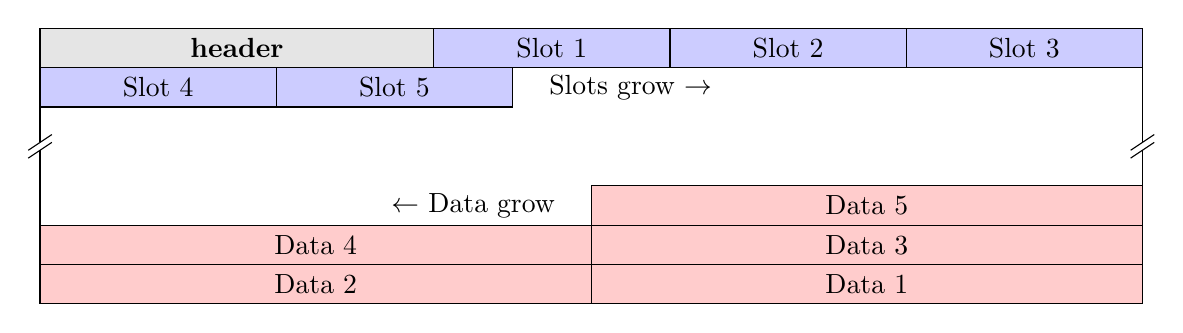
\begin{tikzpicture}
      % Page Outline
      \foreach \x in {0, 14}{
          \draw (\x,0) -- (\x,1.95);
          \draw (\x-0.15,1.85) -- (\x+0.15,2.05);
          \draw (\x,3) -- (\x,2.05);
          \draw (\x-0.15,1.95) -- (\x+0.15,2.15);
        }

      % Header Section
      \fill[gray!20] (0,3) rectangle (5,3.5);
      \node[anchor=center] at (2.5,3.25) {\textbf{header}};
      \draw (0,3) rectangle (5,3.5);

      % Slots Section
      \fill[blue!20] (5,3) rectangle (14,3.5);
      \fill[blue!20] (0,2.5) rectangle (6,3);

      % Slots (Fixed-size entries)
      \foreach \x in {5, 8, 11} {
          \draw (\x,3) rectangle (\x+3,3.5);
          \node[anchor=center] at (\x+1.5,3.25) {Slot \pgfmathparse{(\x-2)/3} \pgfmathprintnumber[precision=0]{\pgfmathresult}};
        }
      \foreach \x in {0, 3} {
          \draw (\x,2.5) rectangle (\x+3,3);
          \node[anchor=center] at (\x+1.5,2.75) {Slot \pgfmathparse{(\x)/3 + 4} \pgfmathprintnumber[precision=0]{\pgfmathresult}};
        }

      \node[anchor=center] at (6+1.5,2.75) {Slots grow $\rightarrow$};

      % Data Section
      \fill[red!20] (7,0) rectangle (14,1.5);
      \fill[red!20] (0,0) rectangle (14,1);

      \foreach \x in {14, 7} {
          \draw (\x,0) rectangle (\x-7,0.5);
          \node[anchor=center] at (\x-3.5,0.25) {Data \pgfmathparse{2-(\x)/7 + 1} \pgfmathprintnumber[precision=0]{\pgfmathresult}};
          \draw (\x,0.5) rectangle (\x-7,1);
          \node[anchor=center] at (\x-3.5,0.75) {Data \pgfmathparse{2-(\x)/7 + 3} \pgfmathprintnumber[precision=0]{\pgfmathresult}};
        }
      \draw (14,1) rectangle (7,1.5);
      \node[anchor=center] at (14-3.5,1.25) {Data \pgfmathparse{2-(14)/7 + 5} \pgfmathprintnumber[precision=0]{\pgfmathresult}};
      \node[anchor=center] at (7-1.5,1.25) {$\leftarrow$ Data grow};

    \end{tikzpicture}}
  \centering
  \caption{Slotted Page grow visualization}
\end{figure}

In our implementation, we only store the tuple count in the header.
We split each tuple to construct our shuffle simulation close to real-world usage.
Each slot contains the 4-byte key together with data offset and length information.
We store the remainder of the tuple in the data section at the end of each page.

As we use fixed-size tuples in our simulation, we only need the tuple slot index to store the tuple on the page.
In contrast, when dealing with variable-size tuples, slot index and data offset are needed to store a tuple.

\section{Slotted Page Managers}\label{section-slotted-page-managers}
As some implementations share the same tuple write-out strategy, we propose the used write-out strategies here and reference them in the following explanations of the concrete implementations.

\begin{table}[h]
  \centering
  \small
  \begin{tabular}{|p{0.19\textwidth}|p{0.40\textwidth}|p{0.30\textwidth}|}
    \hline
    \textbf{Variant}             & \textbf{Tuple Writing}                                                                 & \textbf{Synchronization}                                                                         \\
    \hline
    Lock-based                   & Append to current page; allocate new page if full and append tuple                     & Per-partition lock                                                                               \\\hline
    Lock-free                    & CAS-based index fetch; allocate new page if full after write; insert tuple using index & Per-slotted page tuple index atomic                                                              \\\hline
    Radix-based                  & Pre-allocate pages using global histogram, write independently                         & Synchronisation required when creating global histogram, during page allocation and distribution \\\hline
    Ad-hoc Radix  ("Hybrid")     & Pre-allocate pages using thread-local histogram, write independently                   & Synchronisation required during page allocation and distribution                                 \\\hline
    Thread-Local Pages and Merge & Write to thread local pages; merge non-full pages                                      & Synchronization during local page collection and during partition-range to merge assignment      \\\hline
  \end{tabular}
  \caption{Overview of the Slotted Page Managers}
\end{table}

We initialize each partition with an empty slotted page to simplify the implementations.
Initializing each partition with a slotted page significantly reduces the complexity of the page manager implementations.

\subsection{Lock-based Page Manager}
We use a single lock and a vector for each partition to store the slotted pages.
\begin{algorithm}[h]
  \caption{Lock-based Page Manager insert\_tuple Algorithm}
  \label{Lock-based-page-manager-insert-tuple}
  \SetKwInOut{Input}{input}

  \Input{ \texttt{tuple}: The tuple to be inserted, \texttt{partition}: The target partition index}

  \SetKwFunction{Insert}{insert\_tuple}

  \textbf{function} \Insert{tuple, partition}:

  \textbf{with} partition\_locks[partition]:
  \tcp{Acquire lock}
  \If{\textbf{not} pages[partition][-1].add\_tuple(tuple)}{
    add\_page(partition) \;
    pages[partition][-1].add\_tuple(tuple) \;
  }
\end{algorithm}
As can be seen in Algorithm \ref{Lock-based-page-manager-insert-tuple}, the lock-based insertion process is straightforward.
The insertion on a given slotted page, can only fail if the page is full.
This can easily be checked by reading the tuple count in the metadata section of the slotted page.
If the current page is full, we just allocate and append a new slotted page to the page vector of this partition.

\subsubsection*{Tuple insertion in batches}
Similarly, we can further optimize the write-out by using tuple-batches.
\begin{algorithm}[h]
  \caption{Lock-based Page Manager insert\_tuple\_batch Algorithm}
  \label{Lock-based-page-manager-insert-tuple-batch}
  \SetKwInOut{Input}{input}

  \Input{ \texttt{tuples}: The tuple-batch to be inserted\\ \texttt{partition}: The target partition index}

  \SetKwFunction{Insert}{insert\_tuple\_batch}

  \textbf{function} \Insert{tuples, partition}:

  \textbf{with} partition\_locks[partition]:
  \tcp{Acquire lock}
  \For{tuple \textbf{in} tuples}{
    \If{\textbf{not} pages[partition][-1].add\_tuple(tuple)}{
      add\_page(partition) \;
      pages[partition][-1].add\_tuple(tuple) \;
    }
  }
\end{algorithm}

In Algorithm \ref{Lock-based-page-manager-insert-tuple-batch}, we reuse the tuple insertion logic from Algorithm \ref{Lock-based-page-manager-insert-tuple} but acquire the partition lock only once for the entire insertion process.
Since acquiring and releasing the lock is expensive, this optimization significantly improves performance in multi-threaded scenarios.

\subsection{Lock-free Page Manager}
As holding a lock of a partition denies a second thread to also write out tuples, we propose a lock-free implementation.
Compared to the lock-based variant, we must store our slotted pages in a pointer-stable data structure.
A pointer-stable data structure is necessary to ensure threads can work simultaneously while a thread adds a new slotted page.
Furthermore, we must edit the slotted page metadata using compare-and-exchange operations to avoid losing writes from other threads.

\begin{algorithm}[h]
  \caption{Lock-free Slotted Page increment\_and\_fetch\_opt\_write\_info Algorithm}
  \label{Lock-free-page-increment}
  \SetKwFunction{Increment}{increment\_and\_fetch\_opt\_write\_info}

  \textbf{function} \Increment{}:

  current\_tuple\_count = header->tuple\_count.load()

  \While{\textbf{not} header->tuple\_count.compare\_exchange\_weak(current\_tuple\_count, current\_tuple\_count + 1)}{
    \If{current\_tuple\_count >= get\_max\_tuples(page\_size)}{
      \Return none
    }
  }

  \Return \{page\_ptr, page\_size, current\_tuple\_count\}
\end{algorithm}
In order to gather the information where we can write a tuple, we increment the tuple count using a compare-and-exchange operation.
This previously stored index then acts as our location, where we store the tuple on the page.
In Algorithm \ref{Lock-free-page-increment}, we also add a condition to stop attempting to further increase the count of tuples on the page if it is full.
This condition ensures that threads move to the newly allocated page.
Given the index, where the tuple is placed, we also append a pointer to the start of the page and the page size.
This information ensures we can write the tuple on the page without requiring any further information.

\begin{algorithm}[h]
  \caption{Lock-free Page Manager insert\_tuple Algorithm}
  \label{Lock-free-page-manager-insert-tuple}
  \SetKwInOut{Input}{input}
  \SetKwInOut{Output}{output}

  \Input{\texttt{tuple}: The tuple to be inserted, \texttt{partition}: The target partition index}
  \Output{Tuple inserted into the appropriate slotted page of the specified partition.}

  \SetKwFunction{Insert}{insert\_tuple}

  \textbf{function} \Insert{tuple, partition}:

  wi = current\_page[partition].load().increment\_and\_fetch\_opt\_write\_info()

  \While{\textbf{not} wi}{
    wi = current\_page[partition].load().increment\_and\_fetch\_opt\_write\_info()
  }

  \If{wi.tuple\_index == LockFreeSlottedPage.get\_max\_tuples(wi.page\_size) - 1}{
    add\_page(partition)
  }

  LockFreeSlottedPage.add\_tuple\_using\_index(wi, tuple) \end{algorithm} Using the Algorithm \ref{Lock-free-page-increment}, we retrieve the information to write the tuple in Algorithm \ref{Lock-free-page-manager-insert-tuple}.
We read from an atomically stored pointer to our current page until we receive an index on a slotted page.
If we write the last tuple on the page, we add a new page to this partition.
This last-tuple-check is necessary to create a unique condition when allocating a new page.
With that information, we can write the tuple onto the slotted page.
\subsection{Histogram-based Page Managers}
The following page managers use histograms to keep track of the count of tuples per partition within a given set of tuples.
Similar to Radix Partitioning (see Section \ref{sec-rw-radix-partitioning}), this information can be used to assign memory areas on slotted pages.
\subsubsection{Radix Page Manager} \label{subsubsection-Radix-Page-Manager}
This page manager applies the concept of Radix Partitioning on slotted pages.
It uses a three-step process:
\begin{enumerate}
  \item Histogram retrieval: Each thread reads its assigned materialized tuple chunk and
        builds up a histogram.
        As we are using fixed-size tuples, it only stores the tuple count per partition.
        Then, we forward this histogram to the Radix Page Manager, which collects the histogram of each thread and then moves on to step 2.

  \item Page allocation: With all histograms at hand, the page manager sums up each
        histogram into a global histogram.
        This global histogram stores how many tuples each partition has to store.
        With that information, we can allocate the required pages for each partition.
        When all pages are ready to be used, step 3 begins.

  \item  Assignment of slotted page sub-chunks: Each thread uses its local histogram to
        request storage locations for its tuples.
        The page manager uses the pre-allocated pages to assign each thread one or more memory chunks.
        The thread can then use these memory chunks exclusively to store each tuple.
        Only the tuple count in the metadata has to be atomicly updated once, to signal that this thread has finished its work on this page.
        Otherwise, this write-out process does not rely on synchronization after the memory chunk distribution.
\end{enumerate}
After these three steps, each page can be sent to its receiver once the expected tuple count is reached.
The last thread to atomically-increment the tuple count in the metadata section can do this.

\subsubsection{Ad-hoc Radix ("Hybrid") Page Manager} \label{subsubsection-Ad-hoc-Radix-Page-Manager}
The idea of the previous Radix Page Manager can be used to construct an approach where each thread can hand in its histogram and receive memory chunks on slotted pages independently from other threads.
This page manager merges the three steps of the Radix Page Manager into one.

A thread hands in its histogram and requests the memory chunks, where the tuples can be written.
The page manager reads the histogram and processes each partition individually.
We acquire the partition lock for each partition where at least a single tuple has to be stored.
If there is any space left on a slotted page, it is used up and assigned to this thread.
When the current page is full, we allocate a new page, and the page manager continues the assignment process.
Each thread uses these exclusive memory locations to store its tuples.

Compared to the Radix Page Manager, this page manager does not pre-allocate all necessary pages.
Instead, it allocates the pages when needed.
Furthermore, a thread can already receive its memory chunks while others still construct their histograms.
This change allows this implementation to avoid the materialization of all tuples.
\subsection{Thread-Local Pages and Merge-based Page Manager}\label{subsection-Thread-Local-Pages-Page-Manager}
A further step into reducing the necessity of synchronization is thread-local slotted pages.
We split this slotted page management scheme into two phases:
\begin{enumerate}
  \item Thread-local write-out: These slotted pages are exclusively used by the owning thread, and after the thread finishes its tuple processing, each thread hands in its pages.
        When the page manager receives all pages of each thread, the merging phase starts.

  \item Page merging: The page manager splits all partitions onto the available threads.
        Each thread is then responsible for merging the slotted pages for each partition in the assigned partition range.
        To minimize tuple movement, the slotted pages are sorted decreasingly by the tuple count.
        Then, we merge the pages with fewer tuples into the fuller pages.
        If the last page cannot be fully merged into any other slotted page, then this page has to be reordered so that the slots and data section start at the beginning of the section.
        This reordering is necessary to avoid having a gap at the beginning of the slot or data section.
\end{enumerate}
After the merging phase, this implementation stores all tuples on the least possible number of slotted pages.
During the thread-local processing, this implementation will likely create more slotted pages than necessary.
This unnecessary allocation of pages can lead to a significantly higher memory consumption than the previous approaches.
\subsection{Implementation-independent Optimizations}
We use the following optimizations to speed up our simulation of the shuffle operator.
\subsubsection{Padded atomics and locks}
All implementations that use an array of partition locks are affected by false sharing.
False sharing appears when a cache line stores two independent values and one \ac{CPU} core modifies the first value.
Then, another CPU core wants to access the second value, which causes a cache miss.

We avoid this performance degradation by storing each partition lock aligned to the L1-cache line boundary.
This alignment significantly reduces the number of L1 cache misses, as partition locks are frequently accessed.

\subsubsection{Minimal page-locking}
When holding a partition lock, the tuple write-out onto a slotted page is expensive.
We gather the necessary write-out information to reduce the lock duration, prepare the subsequent tuple insertion, and release the lock before the actual tuple write-out.

\subsubsection{Two-step buffered slotted page write out}
We can process each tuple individually when writing out a batch of tuples onto a slotted page.
First, we construct the slot for the tuple, then store the variable-size data in the data section at the end of the page.
Linux on an x86-64 machine typically uses 4 KiB memory pages.
As we use 5 MiB slotted pages, the slot and data are expected to be on different memory pages.

We store our batches in slot and data phases to reduce the amount of simultaneously accessed pages.
As we now write to the slot or data section, we switch between memory pages less often.
This two-phase approach is more friendly to the \ac{CPU} cache and the \ac{TLB}.

\section{On-Demand Partitioning} \label{section-On-Demand-Partitioning}
\subsection{Overview}
On-demand Partitioning is the most straightforward algorithm for implementing the shuffle operator.
As soon as this implementation receives a batch of tuples, it processes each tuple individually.
First, the hash function is applied to the tuple to gather information on the partition to which this tuple belongs.
With this information, we can write the tuple into the corresponding partition.

This implementation is compatible with the lock-based or lock-free Page Manager and the Thread-Local Pages and Merge-based Page Manager (see Section \ref{section-slotted-page-managers})

\subsection{Software Managed Buffers-based Partitioning}

This naive approach can be significantly improved by using \acfp{SMB}.
Instead of immediately writing out the tuple, we store it in a thread-locally allocated buffer.
Each partition owns a dedicated area within this buffer.
We write the tuples to a slotted page when this sub-region capacity is full.
Similarly, if all incoming tuples have been processed, we write out all remaining tuples inside the buffer.

This temporal storage brings another benefit.
We can now use the batch insertion features from the page managers.
Batch insertions are more \ac{CPU}-cache and \ac{TLB} friendly, as we switch our modified memory locations less often.

\section{Histogram-based Partitioning}\label{section-histogram-based-partitioning}
\subsection{Overview}
Like Radix Partitioning (see Section \ref{sec-rw-radix-partitioning}), we use a histogram to assign threads memory location to store the tuples.
A histogram in the context of Radix Partitioning stores information like the count of tuples and their total size per partition.
We use this information to assign each thread the memory blocks it needs.

In our fixed-size tuple case, we only store the count of tuples of each partition.
As we have to construct the whole histogram, we have to iterate over all tuples twice before the thread can store any tuples.
The first phase is necessary to create the histogram and receive memory locations to store the tuples.
The second phase then uses these memory locations to store the tuples.

Similar to On-Demand Partitioning (see Section \ref{section-On-Demand-Partitioning}), the proposed implementations below benefit from \acfp{SMB} to write out tuples in batches.
\subsection{Radix Partitioning}
This implementation naively implements Radix Partitioning on a stream of incoming tuple batches.
First, we fully materialize all generated tuples.
Then, each thread receives a part of the materialized tuples.
Like in traditional Radix Partitioning, we construct the histogram for the assigned tuples.

The Radix Page Manager (see Section \ref{subsubsection-Radix-Page-Manager}) collects the histograms of all threads.
Each thread then receives its exclusive memory locations to store its tuples.
We can store the tuples without synchronization as we assign exclusive memory locations.
Only the tuple count in the metadata section of each slotted page has to be updated atomically.
A slotted page can be sent to the next downstream operator when it reaches its proposed tuple count.

\subsection{Ad-hoc Radix ("Hybrid") Partitioning}
As the full materialization of all generated tuples and the wait times until the global histogram is created are expensive, we propose a more efficient solution.
Instead of materializing all tuples, we process all incoming tuples morsel-driven.
For a given morsel, we then create a histogram.
The Ad-hoc Radix Page Manager (see Section \ref{subsubsection-Ad-hoc-Radix-Page-Manager}) uses this morsel-histogram to greedily assign this thread exclusive memory location to store the tuples.

Like in the streaming Radix Partitioning case above, we store the tuples on slotted pages without synchronization.
The tuple count in the metadata section also requires synchronization in the form of an atomic tuple count.
As the morsel size is smaller than the materialized tuples' assigned part, we must increase the tuple counter more often than using streaming Radix Partitioning.

\section{Collaborative Morsel Processing}\label{section-Collaborative-Morsel-Processing}
\subsection{Overview}
In the previous implementations, each thread could write to each partition, and we avoided invalid writes by using locks or atomic operations.
Shared usage of locks or atomics causes contention and frequent cache invalidations.

To reduce contention, we assign each thread a partition range.
A thread will only write out a tuple if the partitioning function maps it to a partition within this partitioning range.
Nevertheless, we still have to partition all tuples to their correct partition.
Because of that, we have to process each tuple so that it can end up in any partition.
Thus, we must process each tuple by a group of threads, where the union of their partition ranges covers all possible partitions.
\subsection{Collaborative Morsel Processing with exclusive partition ranges}\label{section-CMP-with_exclusive-partition-ranges}
This implementation constructs the partition ranges so that it fulfills two conditions:
\begin{enumerate}
  \item Any partition range does not overlap with any other partition range.
  \item The union of all partition ranges results in a complete coverage of all possible partitions.
\end{enumerate}
With these two conditions in place, we avoid having to synchronize the tuple write-out process.
However, we must process each tuple $p$ times, where $p$ is the number of partition ranges.
As the incoming tuples only have to be read, they typically can reside in the L2 or L3 \ac{CPU} caches.

Assuming uniform distribution across all partitions, the implementation efficiency decreases with increasing CPU core count.
If we distribute the partitions ($p$) into fair partition ranges, the likelihood of a given tuple being partitioned in a given partition range is:
\begin{equation}\label{equation-CMP-exclusive-partition-ranges}
  \Pr[X=\textrm{partition range}_i] = \frac{|\textrm{partition range}_i|}{p},  \quad \forall i
\end{equation}
As we want to increase the amount of partition ranges with increasing core count, the likelihood that a thread processes a tuple for its assigned partition range decreases.
This is the case, as with increasing partition ranges the sizes of each partition range decreases.
\subsection{Collaborative Morsel Processing using processing units}
As we can see in the above \ac{CMP} with exclusive partition ranges implementation, exclusive partition ranges theoretical performance does not scale well.
This implementation aims to reduce this impact by using processing units.
A processing unit is a partition of $t$ threads that splits the total partitions into $t$ fair, exclusive partition ranges.
Again, within a processing unit, no partition ranges overlap.

When we use multiple processing units, we have to synchronize the tuple write-out again.
In contrast to previous implementations without exclusive partition ranges, each partition can be written by only one thread per processing unit.
This significantly reduces the contention on the synchronization mechanism of each partition.

Furthermore, we must process each tuple only by a single processing unit.
Assuming we fairly split up our $c$ \ac{CPU} cores into $pu$ processing units, then each processing unit will have around $pt\approx\frac{c}{pu}$ threads to process tuples.
When we increase the count of CPU cores and processing units similarly, the amount of threads per processing unit remains constant.
Thus, our likelihood of a randomly selected thread processing a tuple that belongs to its partition range is:
\begin{equation}\label{equation-CMP-PU}
  \Pr[X=\textrm{partition range}_i] \approx \frac{|\textrm{partition range}_i|}{pt},  \quad \forall i
\end{equation}

When we compare the approximation in \ref{equation-CMP-exclusive-partition-ranges} and \ref{equation-CMP-PU}, it is visible that as long as we keep the ratio between CPU cores and processing units constant, the processing efficiency per thread remains constant.
In contrast, when using \acl{CMP} with exclusive partition ranges, the amount of exclusive partition ranges increases with the CPU core count.
This increase in exclusive partition ranges decreases the processing efficiency when increasing the CPU cores.

\section{Thread-Local Pages and Merge-based Partitioning}
This implementation is very similar to the previous On-Demand implementation with \aclp{SMB} (see Section \ref{section-On-Demand-Partitioning}).
Instead of using the On-Demand Page Manager, it heavily builds on the Thread-Local Pages and Merge-based Page Manager (see Section \ref{subsection-Thread-Local-Pages-Page-Manager}).
Thus, this solution avoids sharing slotted pages between threads, which can only be achieved with significantly higher memory usage.

Each thread partitions the incoming tuples into thread-local slotted pages.
With increasing tuple count and more partitions, these thread-local slotted pages are less likely to be fully used, leading to significant memory overhead.
We hand these slotted pages to the shared Page Manager at the end of the tuple processing.

When the Page Manager receives all slotted pages, the slotted pages of each partition are sorted decreasingly by the number of tuples they store.
Then, each thread is assigned an exclusive partition range and slotted pages for this partition range.
All threads then merge the emptier pages into the fuller pages.
All empty pages, which caused the additional memory overhead of this implementation, are then deallocated.
Then, each thread returns the merged slotted pages to the Page Manager, which is the last part of the partitioning process.

\section{Complexity Analysis}
\subsection{Time Complexity}
To shuffle the tuples into partitions, we have to process every tuple.
Thus, $\Omega(n)$ is the lower bound for all shuffle implementations.
As we process each tuple at most $c = \textrm{max}(2, t)$, with $t$ denoting the thread count, times and only apply $O(1)$ operations on each tuple, we can upper bound the implementations time complexity using this constant $O(c * n) = O(n)$.
Combining both lower- and upper bounds, our proposed implementations run in $\Theta(n) = \Omega(n) \cap O(n) $.
\subsubsection{Tuple Access Frequency}
As the theoretical Time Complexity analysis above hides the constant $c = \textrm{max}(2, t)$, we list the tuple access frequency per implementation:
\begin{itemize}
  \item On-Demand Partitioning: Every tuple is only processed once and directly written to its final destination.
        When not using \acp{SMB}, we write each tuple directly onto the slotted page and only access it once.
        In comparison, when using \acp{SMB}, we temporally store the tuple in the buffer, which increases the access count to two.
  \item Histogram-based Partitioning: To create a Histogram, we have to access the tuple once.
        Furthermore, if the implementation requires full materialization, we materialize all tuples before processing them.
        This means that the tuple access frequency is two or three, depending on whether materialization is necessary.

  \item Collaborative Morsel Processing: In the more straightforward implementation with exclusive partition ranges, we have to process each tuple at least $pr$ times, with $pr$ denoting the count of exclusive partition ranges.
        As we use \acp{SMB}, we access each tuple twice when processing it.
        Thus, the tuple access frequency is $2pr$.

        When using processing units, we only have to process at most $\textrm{max}(pt_i), \; \forall i$ times.
        $pt_i$ is the total number of threads (and count of exclusive partition ranges) of processing unit $i$.
        Similarly, it follows that the tuple access frequency is upper bounded by $2 * \textrm{max}(pt_i), \; \forall i$ as we use \acp{SMB} as well.

  \item Thread-Local Pages and Merge-based Partitioning: In this implementation, we also use \acp{SMB}.
        Similar to the On-Demand Partitioning, we must at least store the tuples two times.
        However, as we are using thread-local slotted pages, we may have to merge a slotted page into another page.
        A tuple can only be merged into another page or moved to a different location once.
        Thus, our tuple access frequency is three.
\end{itemize}
\subsection{Space Complexity}\label{section-space-complexity}
Similarly, as in the Time Complexity analysis, we store each tuple at least once.
Thus, we can set a lower bound of $\Omega(n)$.

As the \acfp{SMB} sizes are constant, we can upper bound it by a constant:
\begin{equation}
  c_\textrm{SMB} = (\textrm{Size of a single SMB}) * (\textrm{Thread count})
\end{equation}
Similarly, the LocalPagesAndMerge uses thread-local slotted pages.
The sort-and-merge phase starts when we finish processing the incoming stream of tuples.
All slotted pages of a partition that are not full have to be merged.
During the merge process, some slotted pages can be merged into other slotted pages and deallocated.
These deallocated slotted pages cause an unnecessary memory consumption that can be upper bounded by a constant:
\begin{equation}
  c_\textrm{LPAM} \leq (\textrm{Partition count}) * (\textrm{Thread count}) * (\textrm{Size of a slotted page})
\end{equation}
This constant $c_\textrm{LPAM}$ is independent of the input tuple size, but it can be several GiB big in real-world cases.
When a distributed database system is used, the total size of incoming tuples is significantly higher than the partition and thread count.
Thus, we continue our space complexity analysis with the assumption: $n \gg c_\textrm{LPAM} $

In the full materialization of Radix Partitioning, we create a copy of each tuple to store it on the page.
Otherwise, we only move the tuples until we store them in their final location on a slotted page.
With this information, we can define the upper bound for the Space Complexity to $O(2 * n + c_{SMB} + c_\textrm{LPAM}) = O(n)$.
It follows that the Space Complexity of each implementation is within $\Theta(n) = \Omega(n) \cap O(n) $ .
